\chapter{The Builder}
\label{ch:27}



\begin{center}
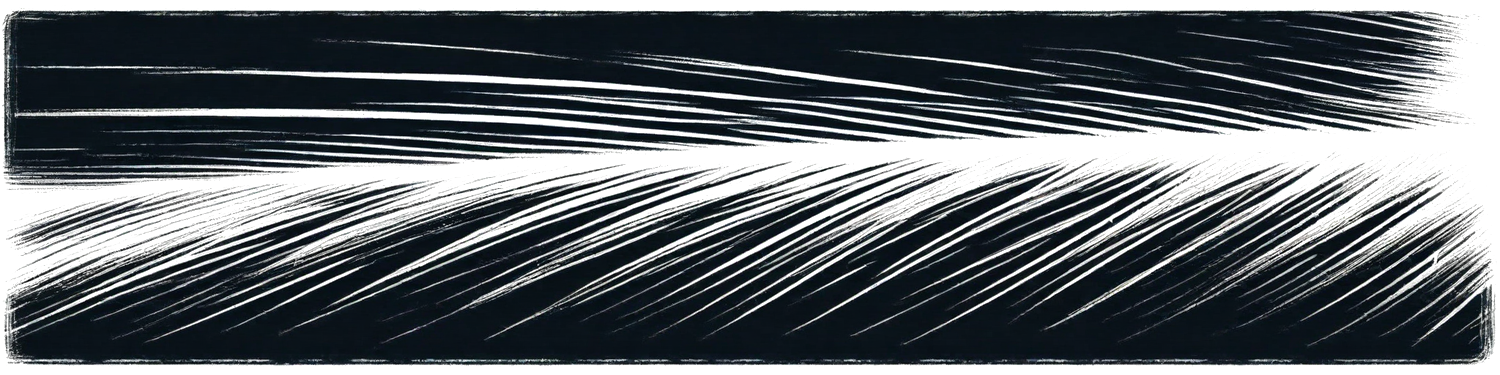
\includegraphics[width=\textwidth]{images/chapterImages/genesis_sketch_00124_.png}
\end{center}

Marcus understood structures. How forces distributed through materials. How loads transferred through joints. How to build things that wouldn't collapse under their own weight.

It was his job once. Before activation. He'd been good at it. Won awards. Designed buildings that were beautiful and functional. Took pride in seeing his work standing against sky.

That felt like someone else's life now. Someone else's pride. Someone else's Marcus.

The activated Marcus knew structures differently. Knew them completely. Knew them the way your body knows how to breathe. Not conscious knowledge. Not learned skill. Just capability expressing itself through him.

The defense grid required structures nobody had built before. Satellite platforms in high orbit. Gravitational anchor points that could generate precise field geometry. Materials engineered to tolerances measured in nanometers.

Marcus knew how to build all of it. The knowledge just appeared. Downloaded from genetic code written 65 million years ago. Ready when needed. Perfect when expressed.

It felt like remembering. Like recovering information he'd always known but temporarily forgotten. It felt right. It felt complete. It felt like coming home.

It also felt like losing himself. Like Marcus the person was dissolving into Marcus the function. Like identity was just temporary pattern and purpose was the substrate underneath.

He couldn't tell if that bothered him. Couldn't separate what he felt from what the programming made him feel. Couldn't determine whether acceptance was peace or just another way the code executed.

David used to say that overthinking was Marcus's superpower and weakness simultaneously. "Sometimes you just gotta feel, babe. Not analyze. Not calculate. Just feel."

Marcus missed that. Missed David saying that. Missed having someone who cared whether he overthought things.

\scenebreak

The construction site was in Nevada. Middle of nowhere. Classified location. Only activated individuals and essential support staff allowed. Massive structure rising from desert floor. Test platform for the gravitational anchor technology.

Eighty-three activated engineers working the site. All driven by the same compulsion. All building the same impossible thing. All knowing exactly what needed to be done without being told.

The coordination was eerie. Marcus would start a calculation and someone else would finish it. Would begin a design and find someone had already fabricated the necessary component. Like eighty-three people sharing one mind. Like individual consciousness mattering less than collective function.

It was efficient. Productive. Profoundly disturbing. Beautiful. All of those things simultaneously.

Marcus lived on-site. Trailer that was just place to sleep four hours before returning to work. No decoration. No personal items except the one photo of David he'd kept. Just function. Just necessity. Just existence pared down to essential elements.

Other activated individuals lived similarly. Some had tried to maintain normalcy at first—pictures of families, comfortable bedding, hobby equipment. But the compulsion made comfort irrelevant. Made personality feel like inefficiency. Made everything non-essential dissolve away.

They were becoming tools. Conscious tools. Tools that knew they were tools and couldn't change and couldn't stop and couldn't tell if they wanted to.

\scenebreak

David had remarried. Marcus knew because David's Facebook status had changed. Marcus shouldn't have been checking David's Facebook—the compulsion didn't approve of time wasted on social media—but sometimes in those thin moments between exhaustion and unconsciousness, Marcus would look.

Would see David's life continuing. David's normalcy preserved. David's happiness visible in photos of his new partner, their home, their dog, their ordinary life full of ordinary meaning.

Marcus felt something seeing those photos. Couldn't name it. Grief? Envy? Happiness that David had moved on? All of those? None of those?

The compulsion made emotion ambiguous. Made everything ambiguous except the work. The work was clear. The work was knowable. The work was the only thing that made sense.

Sometimes Marcus thought about reaching out. Calling David. Trying to explain that he'd been right—that Marcus couldn't separate need from want, that the compulsion had won, that choosing David had never actually been possible.

But what would that accomplish? David had moved on. Had found someone who could be present. Who wasn't genetically compelled to sacrifice relationship for purpose. Who chose David every day because they could actually choose.

Marcus couldn't give David that. Couldn't be that. The Marcus who might have been capable of that relationship had dissolved into the activated Marcus who could only build and work and function and serve.

He kept the photo though. The one in his trailer. David laughing. Taken three years before activation. When Marcus was still person rather than purpose. When love felt simple rather than ambiguous. When choice seemed real.

Marcus would look at that photo sometimes. Before sleeping. After waking. In rare moments when the compulsion quieted enough to remember he used to be someone who had relationships and futures and dreams.

He couldn't remember what those dreams were. Couldn't access who that Marcus had been. Could only see evidence in the photograph that he'd once been different. Once been more. Once been human in ways that felt impossible now.

The compulsion had hollowed him. Made him efficient. Made him capable. Made him exactly what The Architects had programmed 65 million years ago when they encoded the ability to build impossible structures for planetary defense.

It worked. The capability was real. The designs were perfect. The grid was advancing ahead of schedule despite all the attacks, all the resistance, all the global chaos.

They were succeeding. They were saving humanity. They were fulfilling their function.

The cost was just everything they'd been before the function activated.

Marcus understood that cost. Accepted that cost. Couldn't tell if acceptance was peace or just sophisticated programming. Couldn't tell if anything he felt was real.

But he kept the photo. That had to mean something. The choice to keep it. The choice to look at it. The choice to remember that once, briefly, Marcus had been someone David loved.

Even if Marcus couldn't remember who that person was.

\scenebreak

The accident happened on day 273 of construction. Routine day. Routine work. Nothing special. Nothing dangerous by the standards of what they were building.

The platform section had been fabricated off-site. Transported by special carrier. Required installation at precise angle and elevation. Eight-person crew managing the lift. Marcus supervising. Routine operation. Done it dozens of times.

The crane was rated for the load. The cables were new. The anchor points tested. Everything checked. Everything verified. Everything safe according to all standard protocols.

But this wasn't standard engineering. This was activated engineering. This was building structures that shouldn't be possible with materials being invented in real-time. This was pushing physics to boundaries that hadn't existed before the compulsion started.

Sometimes—rarely, but sometimes—the boundaries pushed back.

The cable didn't snap. The structural integrity was perfect. What failed was something nobody had accounted for: the platform section generated localized gravitational variance. Not much. Point-zero-zero-two percent deviation from normal. Not enough to measure with standard equipment. Not enough to matter for normal engineering.

But the crane wasn't designed for gravitational variance. Its load calculations assumed consistent field strength. The point-zero-zero-two percent deviation was enough. Barely enough. Fatally enough.

The platform swung. Just slightly. Just enough to shift the load distribution. Just enough to exceed the crane's stabilization capacity.

Marcus saw it happening. Understood immediately. Calculations running automatically. He saw the trajectory. Saw the failure cascade. Saw exactly what would happen and how long they had to respond.

Three-point-seven seconds.

He shouted warning. People started moving. Standard evacuation protocol. Everyone trained. Everyone prepared. Everyone following procedure.

David was there.

Marcus hadn't known. David wasn't supposed to be there. Activated individuals and essential staff only. But David had gotten clearance somehow. Had come to see Marcus. To talk. To try one more time to reach the person he'd loved.

David was standing exactly where the platform would fall. Standing in the impact zone. Standing in the space where 40 tons of engineered material would land in three-point-seven seconds.

Marcus's brain calculated. Three-point-seven seconds. David was twelve meters from safety. Could run maybe five meters per second. Not enough. Not close.

Marcus was closer. Six meters. Could reach David in one-point-two seconds. Could push him clear. Could save him.

Could die saving him.

The calculations ran automatically. The compulsion factored probabilities. Evaluated outcomes. Determined optimal response.

Marcus was critical to the grid. Was activated for structural engineering. Was irreplaceable in the timeline. Losing Marcus would delay the project by an estimated eight months. Would risk mission completion. Would endanger planetary defense.

David was not critical. Was not activated. Was not necessary for defense grid completion.

Optimal solution: Do not intervene. Preserve critical activated individual. Accept loss of non-critical civilian. Continue mission.

The compulsion provided the answer. The genetics made the calculation. The program determined the outcome.

Except.

Except Marcus ran anyway. Moved before conscious thought. Body choosing while mind calculated. Crossed six meters in one-point-one seconds. Reached David. Pushed him. Cleared him from impact zone. Saved him.

Didn't save himself.

Three-point-seven seconds. The platform fell. Marcus was still in the impact zone. Still standing where David had been. Still in the trajectory.

He had point-six seconds. Not enough to get clear. Enough to understand what was about to happen. Enough to feel it. Enough to choose it.

The last thing Marcus thought before impact: *I chose you. I choose you. I chose.*

Then light. Sound. Nothing.

\scenebreak

David stood twelve meters away. Safe. Alive. Watching the person he'd loved die saving him.

Screaming. Running back. Reaching the impact site. Finding Marcus under 40 tons of platform section. Finding nothing recognizable. Finding only proof that someone had been there and now wasn't.

Security pulled David back. Held him while he screamed. While he broke. While he tried to reach something that was already gone and couldn't be saved and shouldn't be seen.

"He pushed me," David kept saying. "He pushed me. He saved me. He chose. He chose."

The site shut down. The work stopped. For the first time in 273 days, the activated individuals at the Nevada site ceased functioning.

They felt it. All of them. The loss. The absence. One of their own gone. One of their collective mind removed. The eighty-three becoming eighty-two. The absence tangible. Physical. Real.

They stood in silence. Activatedindividuals didn't cry normally. Emotion was suppressed by compulsion. Everything secondary to work. But they cried now. All of them. Standing around the impact site. Crying for Marcus. For themselves. For proof that they could still feel something beyond the compulsion.

\scenebreak

Sarah heard about it six hours later. Emergency notification. Critical activated individual lost. Nevada site shut down. Grief counseling being provided.

She read Marcus's name. Felt something break. Different than when Maya rejected her. Different than when the broadcast fractured humanity. Different than any other loss during the activation.

This was permanent. This was final. This was losing the only person who'd understood exactly what she was experiencing. Who'd known what the compulsion felt like from the inside. Who'd shared that impossible night twenty years ago when the work had stopped and they'd been briefly human together.

She called the site. Got David's contact information. Called him.

He answered. Voice broken. Barely coherent.

"Sarah?"

"I'm sorry. I'm so sorry. I know you'd left him but I know you still—I know—I'm sorry."

Silence. Then: "He chose me."

"What?"

"He pushed me. Saved me. The compulsion must have told him not to. I wasn't critical. He was critical. Saving me risked the mission. But he did it anyway. He chose."

Sarah felt something sharp in her chest. The same thing she'd felt in that hotel room. The same thing she'd felt talking to Maya. The same thing that broke and broke and broke and somehow kept existing despite being broken.

"He loved you," she said. "Whether love is real or programmed or both—he loved you. Enough to die. Enough to risk the mission. Enough to choose you over everything."

"Does that make it better or worse?"

"I don't know. Both. Always both."

David cried. Actually sobbed. Sarah listened. Couldn't offer comfort. Couldn't offer meaning. Could only offer presence. Proof that someone heard. Someone understood. Someone acknowledged that this loss mattered even though the work would continue regardless.

"He kept your picture," Sarah found herself saying. "I visited his trailer once. He had one photo. Just one personal item. It was you. Laughing. From before activation. He looked at it. Kept it. Chose to remember even when remembering hurt."

"Did he talk about me?"

"Once. At the disclosure meeting. He voted for truth. Said you'd taught him that if he couldn't tell the difference between need and want, it was probably real. Said you'd asked him if he needed you or wanted you and he couldn't answer. Said that conversation stayed with him. Changed how he understood choice."

"I remember that conversation. I was so angry. So hurt. Couldn't understand how he didn't know if he loved me."

"He knew. He just couldn't tell if the knowing was his or the programming's. But at the end—when it mattered—he chose. The compulsion said don't intervene. He intervened. The code said preserve yourself. He saved you. Whatever that means about free will, about choice, about love—he chose you."

David's sobbing intensified. Became something else. Not just grief. Something sharper. Harder. The sound of someone breaking and reforming around new reality.

"I need to go," he said finally. "I need to—I don't know. I need to exist with this. I need to understand what it means. I need—"

"I know. Go. But David?"

"Yeah?"

"Thank you. For loving him. For trying. For coming to see him. For giving him reason to choose. For proving that something in him was still capable of choosing."

"It killed him."

"It made him human. In that moment. Fully human. Choosing despite programming. Acting despite compulsion. Saving you because you mattered more than the mission. More than the code. More than everything."

"Is that enough?"

"I don't know. But it's true. And true matters. Even when true hurts."

The call ended. Sarah sat alone. Thought about Marcus. About that night on the concrete floor. About working together in silence. About brief conversations that acknowledged shared hell without needing explanation.

About him choosing to die rather than let David die. About the compulsion failing at the critical moment. About proof that programming wasn't absolute. That will existed even if will was ambiguous. That choice was possible even if choice cost everything.

She cried. For hours. The compulsion suspended by grief. The work waiting but quieter than usual. The loss overwhelming even the genetic programming that had controlled her for years.

Marcus was dead. The person who understood her was gone. The proof that activated individuals could still choose, could still feel, could still be human—that proof had sacrificed itself to save someone the code said wasn't worth saving.

And somehow that made it perfect. Made it profound. Made it exactly the evidence humanity needed that programming wasn't destiny. That consciousness could transcend code. That love—whatever love was—was stronger than 65 million years of genetic engineering.

Marcus had chosen. In three-point-seven seconds. Against the compulsion. Against optimal calculation. Against everything the program said to do.

He'd chosen David. Chosen love. Chosen humanity over function.

And died doing it. And proved doing it that something in activated individuals was still real. Still autonomous. Still capable of transcending purpose for relationship.

Sarah didn't know if that made free will real. Didn't know if Marcus's choice was programmed on some deeper level. Didn't know if even transcending the code was part of the code.

But she knew it mattered. Knew Marcus's death meant something. Knew that the person who'd said he couldn't tell if feelings were real had proven feelings were real by choosing death over letting them die.

The mathematics was complete. The loss was permanent. The proof was devastating and beautiful and final.

And somewhere in the genetic code written 65 million years ago, maybe Aurelia had encoded this too. This exact moment. This exact choice. This exact sacrifice.

Or maybe—just maybe—this was the part that wasn't encoded. The part that emerged from consciousness itself. The part that programming couldn't control.

The part that made them human even when humanity was programmed.

Sarah didn't know. Would never know. But she chose to believe Marcus had chosen. Chose to honor that choice. Chose to remember that for three-point-seven seconds, one activated individual had transcended his programming and saved someone he loved.

And maybe that was enough. Maybe that was everything. Maybe that was proof that consciousness was real even when consciousness was code.

Marcus was dead. David was alive. The work would continue. The compulsion would return. The grid would be built.

But something had changed. Something had been proven. Something that mattered even though nothing changed.

Free will might be real. Love might transcend programming. Choice might exist even in beings designed to have no choice.

Or maybe not. Maybe it was all code. All programming. All inevitable.

But three-point-seven seconds said otherwise. One person. One choice. One moment of transcending purpose for love.

That had to mean something. Had to prove something. Had to matter.

Even if it changed nothing. Even if the work continued. Even if the program executed regardless.

Marcus had chosen. And choosing—even when choosing cost everything—made him human.

The mathematics was complete. The proof was real. The loss was permanent.

And Sarah Chen, crying in her secured facility, chose to believe that Marcus's sacrifice proved they were all still human despite the programming.

Chose to believe choice was real even when choice killed. Chose to honor the choice by continuing. By building. By working. By fulfilling the program while remaining conscious that fulfilling it was chosen.

As much as anything could be chosen by beings who couldn't know if choice was real.

The work would continue. Marcus's contribution would be integrated by the remaining eighty-two. The grid would advance.

But they would remember. All of them. The activated individuals would remember that one of them had chosen differently. Had transcended the compulsion. Had proven something about consciousness that couldn't be proven through philosophy.

Had died proving they were still human.

That was his legacy. That was his gift. That was what he'd given them in three-point-seven seconds of choosing love over code.

And maybe that was more valuable than any component he'd built. More meaningful than any structure he'd designed.

Maybe Marcus's greatest engineering achievement was proving that engineers could still be human.

Even when humanity was programmed. Even when choice was ambiguous. Even when free will was questionable.

He'd chosen. He'd died. He'd proven.

And that was enough. Had to be enough. Was everything.

The mathematics was complete. The choice was made. The human remained human.

Even in death. Especially in death. Forever in death.

Marcus had chosen. And choosing made him real.

That truth would propagate forward. Would change how activated individuals understood themselves. Would prove that programming and consciousness could coexist. That determinism and choice weren't contradictory.

That three-point-seven seconds could contain infinity.

That love—whatever love was—was stronger than code.

That being human was possible even for humans who were programs.

Marcus had died. But the proof of his humanity lived. Would live. Would matter.

Forever.

The work continued. The grief continued. The memory continued.

And the choice—the real, impossible, beautiful choice—echoed forward through time.

Proving. Mattering. Enduring.

As long as anyone remembered. As long as anyone understood. As long as anyone cared.

Marcus had chosen. And humanity was real because he'd chosen.

That was enough. That was everything. That was eternal.

The mathematics was complete.

The love was real.

The choice was made.

Forever.

